\subsubsection{ln 3}\label{sssec:ln3}
 
\zadatak
U {\cv}ast Nepera i Brigsa,
pomo{\cc}u postupka \eqref{eq:alg} sa 
strane~\pageref{eq:alg},
izra{\cv}unaj {\sl pe{\sv}ke\/} pribli{\zv}nu vrednost $\ln 3$
u~5 koraka. Za upore{\dj}iva{\nj}e, ta{\cv}na vrednost je
$$
\ln3=1\.
0986122886\,
6810969139\,
5245236922\,
5257046475\,\ldots
%1639157/1492025=1.098612288668
$$

\def\step#1{\par\indent\leavevmode
  Korak~{\it#1}.\kern2em\relax}

\resenje
Za $x=3$, izraz $r=(x-1)/(x+1)=1/2$. U nultom koraku postav{\lj}amo po{\cv}etne vrednosti:

\smallskip

\step0 $k=1,\quad p=2r=1,\quad q=r^2=1/4,\quad a=p=1,\quad y=a=1$.

\smallskip

\noindent Slede koraci iteracije --- pove{\cc}amo $k$ za 2, pomno{\zv}imo $p$ sa $q$,
{\cv}lan sume $a$ postaje $p/k$, koga dodajemo u rezultat $y$:

\smallskip

\step1 $k=3,\quad p=1/4,\quad a=1/12,\quad y=13/12$;
\step2 $k=5,\quad p=1/16,\quad a=1/80,\quad y=263/240$;
\step3 $k=7,\quad p=1/64,\quad a=1/448,\quad y=7379/6720$;
\step4 $k=9,\quad p=1/256,\quad a=1/2304,\quad y=88583/80640$;
\step5 $k=11,\quad p=1/1024,\quad a=1/11264,\quad y=3897967/3548160$.

\smallskip

\noindent Rezultat je
$$
\ln3\approx\frac{3897967}{3548160}\approx \ram{1\.0986},
$$
{\sv}to nije lo{\sv}e za samo 5 koraka, jer je apsolutna gre{\sv}ka oko $2\.4\puta10^{-5}$.
Ali, mo{\zv}e bo{\lj}e\dots

\dodatak
Ako ve{\cc} imamo precizno izra{\cv}unatu konstantu $\ln2$, onda je bo{\lj}e ra{\cv}unati $\ln3$ kao $\ln(3/4)+2\ln2$,
jer {\cc}e u postupku, umesto $r=1/2$, biti $r=(3/4-1)/(3/4+1)=-1/7$, 
odnosno, umesto $q=1/4$, bi{\cc}e $q=1/49$,
{\sv}to dovodi do mnogo br{\zv}eg izra{\cv}unava{\nj}a. U~istom broju koraka bismo dobili
$$
\ln\frac34\approx
-\ff2/7, -\ff296/1029, -\ff72526/252105, -\ff24876448/86472015, 
-\ff522405418/1815912315, -\ff281576520392/978776737785,
$$
gde posled{\nj}i razlomak ima gre{\sv}ku od oko $1\.6\puta10^{-12}$,
{\sv}to je vi{\sv}e od dvostruko ta{\cv}nih cifara.
Kada mu dodamo $2\ln2$ (vidi stranu~\pageref{ln2}), dobi{\cc}emo
$$\ln3\approx \underbrace{1\.09861228866}_{\hbox{\scriptsize ta{\cv}ne cifre}}\!9726\ldots$$

Generalno, ovakav na{\cv}in je najbr{\zv}i ako ra{\cv}unamo $\ln x=\ln(x/2^n)+n\ln2$,
gde biramo $n$ takvo da $x/2^n$ bude {\sv}to bil{\zv}e 1, odnosno, da $q$ bude najma{\nj}e mogu{\cc}e (vidi program).
$$
\slika{\hbox to 0pt{\hss\hbox{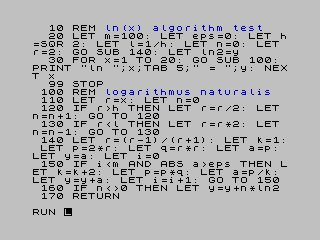
\includegraphics[width=\zxscreen]{eps/ln-prog.png}\enspace
  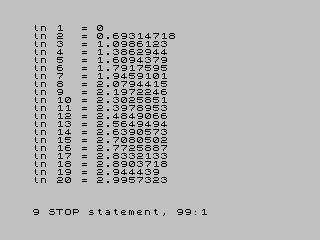
\includegraphics[width=\zxscreen]{eps/ln-run.png}}\hss}}{\textsf{ZX Spectrum} {\BASIC} program.}
$$


% \begin{wrapfigure}{r}{\zxscreen}
% \includegraphics[width=\zxscreen]{eps/ln.png}\\
% \hbox to \zxscreen{\hss \newpic{\textsf{ZX Spectrum} {\BASIC} program.} \hss}
% \end{wrapfigure} 
% Generalno, ovakav na{\cv}in je najbr{\zv}i ako ra{\cv}unamo $\ln x=\ln(x/2^n)+n\ln2$,
% gde biramo $n$ takvo da $x/2^n$ bude {\sv}to bil{\zv}e 1, odnosno, da $q$ bude najma{\nj}e mogu{\cc}e.
